%package list
\documentclass{article}
\usepackage[top=3cm, bottom=3cm, outer=3cm, inner=3cm]{geometry}
\usepackage{graphicx}
\usepackage{url}
%\usepackage{cite}
\usepackage{hyperref}
\usepackage{array}
%\usepackage{multicol}
\newcolumntype{x}[1]{>{\centering\arraybackslash\hspace{0pt}}p{#1}}
\usepackage{natbib}
\usepackage{pdfpages}
\usepackage{multirow}
\usepackage{multirow}
\usepackage[normalem]{ulem}
\useunder{\uline}{\ul}{}



%%%%%%%%%%%%%%%%%%%%%%%%%%%%%%%%%%%%%%%%%%%%%%%%%%%%%%%%%%%%%%%%%%%%%%%%%%%%
%%%%%%%%%%%%%%%%%%%%%%%%%%%%%%%%%%%%%%%%%%%%%%%%%%%%%%%%%%%%%%%%%%%%%%%%%%%%
\newcommand{\csemail}{vmachacaa@ulasalle.edu.pe}
\newcommand{\csdocente}{MSc. Vicente Enrique Machaca Arceda}
\newcommand{\cscurso}{Fundamentos de Lenguajes de
Programación}
\newcommand{\csuniversidad}{Universidad La Salle}
\newcommand{\csescuela}{Escuela Profesional de Ingeniería de Software}
\newcommand{\cspracnr}{03}
\newcommand{\cstema}{Ensamblador}
%%%%%%%%%%%%%%%%%%%%%%%%%%%%%%%%%%%%%%%%%%%%%%%%%%%%%%%%%%%%%%%%%%%%%%%%%%%%
%%%%%%%%%%%%%%%%%%%%%%%%%%%%%%%%%%%%%%%%%%%%%%%%%%%%%%%%%%%%%%%%%%%%%%%%%%%%


\usepackage[english,spanish]{babel}
\usepackage[utf8]{inputenc}
\AtBeginDocument{\selectlanguage{spanish}}
\renewcommand{\figurename}{Figura}
\renewcommand{\refname}{Referencias}
\renewcommand{\tablename}{Tabla} %esto no funciona cuando se usa babel
\AtBeginDocument{%
	\renewcommand\tablename{Tabla}
}

\usepackage{fancyhdr}
\pagestyle{fancy}
\fancyhf{}
\setlength{\headheight}{30pt}
\renewcommand{\headrulewidth}{1pt}
\renewcommand{\footrulewidth}{1pt}
\fancyhead[L]{\raisebox{-0.2\height}{
\includegraphics[width=3cm]{img/logo_salle}}}
\fancyhead[C]{}
\fancyhead[R]{\fontsize{7}{7}\selectfont	\csuniversidad \\ \csescuela \\ \textbf{\cscurso} }
\fancyfoot[L]{MSc. Vicente Machaca}
\fancyfoot[C]{\cscurso}
\fancyfoot[R]{Página \thepage}

\usepackage{listings}
\usepackage{xcolor} % for setting colors

% set the default code style
\lstset{
    frame=tb, % draw a frame at the top and bottom of the code block
    tabsize=4, % tab space width
    showstringspaces=false, % don't mark spaces in strings
    numbers=left, % display line numbers on the left
    commentstyle=\color{green}, % comment color
    keywordstyle=\color{blue}, % keyword color
    stringstyle=\color{red} % string color
}






\begin{document}
	\nocite{10.5555/1610485}
	\vspace*{10px}
	
	\begin{center}	
		\fontsize{17}{17} \textbf{ Práctica \cspracnr}
	\end{center}
	%\centerline{\textbf{\underline{\Large Título: Informe de revisión del estado del arte}}}
	%\vspace*{0.5cm}
	

	\begin{table}[h]
		\begin{tabular}{|x{4.7cm}|x{4.8cm}|x{4.8cm}|}
			\hline 
			\textbf{DOCENTE} & \textbf{CARRERA}  & \textbf{CURSO}   \\
			\hline 
			\csdocente & \csescuela & \cscurso    \\
			\hline 
		\end{tabular}
	\end{table}	
	
	
	\begin{table}[h]
		\begin{tabular}{|x{4.7cm}|x{4.8cm}|x{4.8cm}|}
			\hline 
			\textbf{PRÁCTICA} & \textbf{TEMA}  & \textbf{DURACIÓN}   \\
			\hline 
			\cspracnr & \cstema & 3 horas   \\
			\hline 
		\end{tabular}
	\end{table}
	
	
	\section{Datos de los estudiantes}
	\begin{itemize}
		\item GIT: \href{https://github.com/Robertohg/FLP}{GIT-Repo}
		\item Integrantes: 
		\begin{itemize}
			\item Roberto Heredia Garland
			
		\end{itemize}		
	\end{itemize}
	
	
	

	
	\section{Ejercicios}\label{sec:ejercicios}
	\begin{enumerate}
		\item Implementar un programa que muestre la suma, la diferencia, la multiplicación, la división y el promedio de dos números ingresados por teclado.
	

	
		\begin{lstlisting}[language={[x86masm]Assembler}, basicstyle=\small]

.data
    txt1: .asciiz "\nIngrese un numero \n"
    txt2: .asciiz "\nIngrese otro numero \n"
    suma: .asciiz "\nLa suma es \n"
    dif: .asciiz "\nla diferencia es \n"
    multi: .asciiz "\La multiplicacion es o\n"
    divi: .asciiz "\La divicion es o\n"
.text
main:
	la $a0, txt1
	li $v0,4
	syscall

	li $v0,6 #f0
	syscall

	mov.s	$f1, $f0
	la $a0, txt2
	li $v0,4
	syscall

	li $v0,6 #f0
	syscall

	mov.s	$f2, $f0
	add.s $f12, $f2, $f1 #sumar
	mov.s $f13, $f12
	la $a0, suma
	li $v0,4
	syscall

	li $v0,2
	syscall

	sub.s $f12, $f1, $f2 
	la $a0, dif     #restar
	li $v0,4
	syscall

	li $v0,2
	syscall

	mul.s $f12, $f1, $f2 
	la $a0, multi       #multiplicar
	li $v0,4
	syscall

	li $v0,2
	syscall

	div.s $f12, $f1, $f2 
	la $a0, divi        #dividir
	li $v0,4
	syscall

	li $v0,2
	syscall


	jr	$ra
		   \end{lstlisting}
	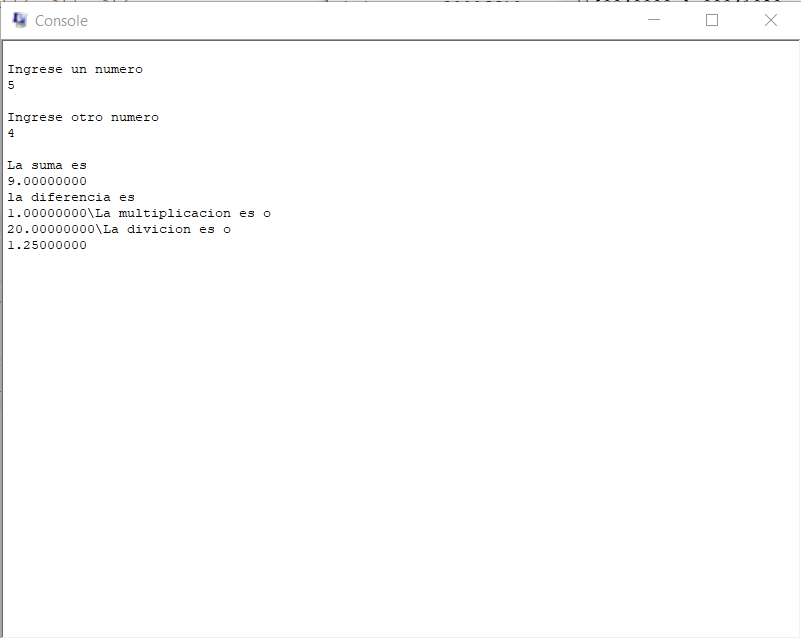
\includegraphics[width=8cm]{img/eje1.png}
	\newpage
	\item Implementar un programa que solicite una cantidad \textit{n} de números y luego retorne: la suma de estos, el promedio, el mayor y el menor.
	
		\begin{lstlisting}[language={[x86masm]Assembler}, basicstyle=\small]

.data 
	ingrese_numero: .asciiz "Ingrese el numero de iteraciones: "
	numero_mayor: .asciiz "El numero mayor : "
	numero_menor: .asciiz "\nEl numero menor : "
	promedio: .asciiz "\nEl promedio : "
	numero: .asciiz "Ingrese el numero : "

.text 
main: 	
	
	li $t1,0
	li $t2,0 
	li $t3,0 
	li $t4,0 
	li $t5,0  
	
	
	li $v0, 4 				
	la $a0, ingrese_numero 		
	syscall 			
	
	
	li $v0,5
	syscall
	
	
	move $t2,$v0 
	
	li $v0, 4 				
	la $a0, numero 		
	syscall 	
	li $v0,5
	syscall
	
	add $t5, $t5, $v0
	
	
	move $t3,$v0
	move $t4,$v0
	
	add $t1,$t1,1   
	
	Loop:
		beq $t2,$t1, Exit
		
		li $v0, 4 				
		la $a0, numero 		
		syscall 
		li $v0,5
		syscall
		
		add $t5, $t5, $v0
				
		
		bgt $v0, $t3, Them1
			j EndIf1
		Them1:
			move $t3, $v0
		EndIf1:
		
		bgt $t4, $v0, Them2
			j EndIf2
		Them2:
			move $t4, $v0
		EndIf2:	
		
		add $t1,$t1,1  
			
		
		j Loop
	Exit:		
	
	li $v0, 4 				
	la $a0, numero_mayor 		
	syscall 
	
	move $a0, $t3
	li $v0, 1 
	syscall
		
	li $v0, 4 				
	la $a0, numero_menor 		
	syscall 
	
	move $a0, $t4
	li $v0, 1 
	syscall
		
	li $v0, 4 				
	la $a0, promedio		
	syscall 
		
	mtc1 $t5, $f0
	cvt.s.w $f0, $f0

	mtc1 $t2, $f1
	cvt.s.w $f1, $f1
	
	div.s $f12, $f0, $f1
	li $v0, 2 
	syscall
		
	jr $ra
		   \end{lstlisting}	
	
	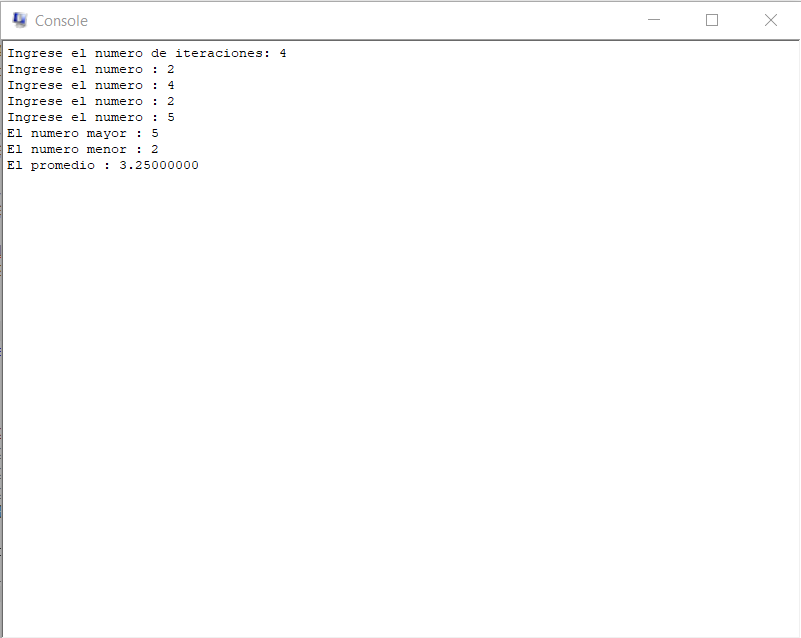
\includegraphics[width=8cm]{img/eje2.png}
	
	\clearpage
	%\bibliographystyle{apalike}
	%\bibliographystyle{IEEEtranN}
	%\bibliography{bibliography}
		\end{enumerate}
	
\end{document}